

\exercise{Abstract MSF}{2}
A dynamical system has a steady state whose Jacobian matrix is given by
\eq{
{\bf P}=\avecc{2 & 3 \\ -3 & -4} 
}
We place copies of this system in the nodes of a network and couple them diffusively such that the coupling matrix is 
\eq{
{\bf C} = \avecc{1 & 0 \\ 0 & 10}
}
Compute and sketch the master stability function for this system. Describe what the result means for the network. 

\solution

Using the results from the stability is determined by the eigenvalues of 
\eq{
{\bf J} =\avecc{2 & 3 \\ -3 & -4} - \kappa  \avecc{1 & 0 \\ 0 & 10} = \avecc{2-\kappa & 3 \\ -3 & -4-10\kappa}
}
By the (somewhat tedious) factorization of the characteristic polynomial we find 
\eqa{
\lambda_1 &=& -1 - \frac{11}{2} k + \frac{3}{2} \sqrt{9\kappa^2+12\kappa} \\
\lambda_2 &=& -1 - \frac{11}{2} k - \frac{3}{2} \sqrt{9\kappa^2+12\kappa} 
}
Both eigenvalues are real and the first one is the greater one. Therefore the master stability function is 
\eq{
M(\kappa) = -1 - \frac{11}{2} k + \frac{3}{2} \sqrt{9\kappa^2+12\kappa} 
}
which looks like this
\begin{center}
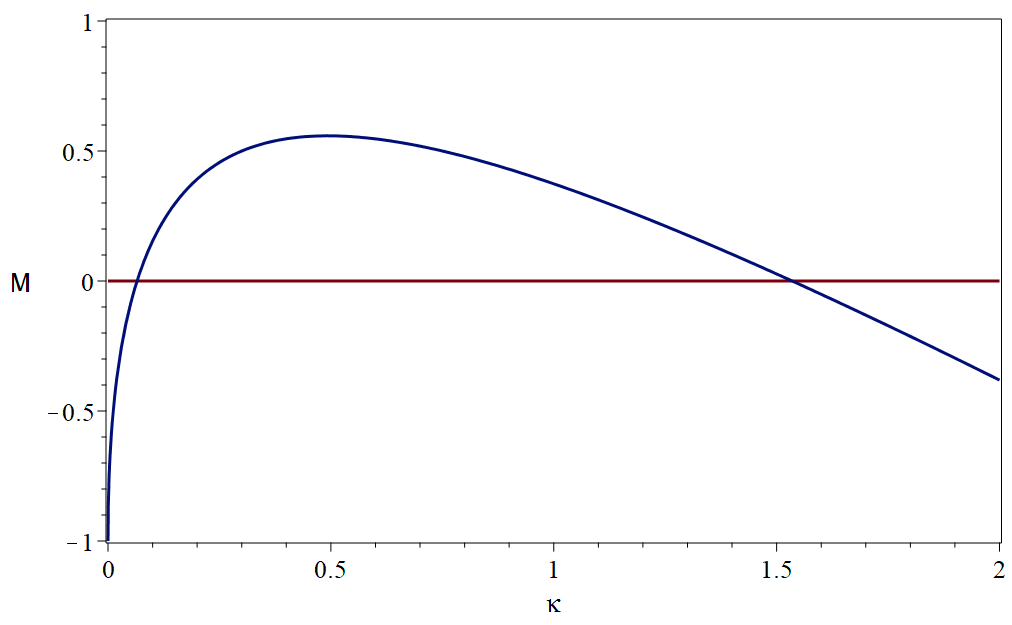
\includegraphics[width=0.6\textwidth]{MSF}
\end{center}
We can see that there is a positive region. To find this region exactly 
we can solve 
\eq{
0 = -1 - \frac{11}{2} k + \frac{3}{2} \sqrt{9\kappa^2+12\kappa} 
}
yields the solutions
\eqa{
\kappa_1 &=& \frac{4}{5} - \frac{3}{10} \sqrt{6} \approx 0.07\\
\kappa_2 &=& \frac{4}{5} + \frac{3}{10} \sqrt{6} \approx 1.53
}
So in summary the homogeneous steady state under consideration is stable if the Laplacian matrix of the network does not have an eigenvalue with value $\kappa$ between 0.07 and 1.53. In practice this means that the system is stable if the spectral gap eigenvalue (the second smallest eigenvalue) must be at least 1.53.  
